\chapter{Theory}\label{chapter:theory}
\section{The Standard Model}\label{sec:sm}
The Standard Model (SM) of particle physics is a theory which describes all the known elementary particles and their interactions with the weak, strong, and electromagnetic forces through a renormalisable Quantum Field Theory (QFT).

All matter is described as spin-$\frac{1}{2}$ particles known as fermions and the fundamental forces are mediated by spin-$1$ gauge bosons.
The spin-$0$ Higgs boson arises as a consequence of the electroweak symmetry breaking as a means to imbue the fermions and Weak gauge bosons with mass.

Matter consists of three ``generations''  of two types of fermion

\begin{table}[htbp]
\topcaption {
The Standard Model fermions and their properties.
}
\label{tab:fermions}
  \centering
  \resizebox{\textwidth}{!}{
% This right-aligns numbers in column, but centers them under column title.
 \begin{tabular}{llcllccc}
   \hline
   & \textbf{Generation} & \textbf{Particle} & & \textbf{Mass \MeV} & \textbf{Electric Charge} & \textbf{Colour Charge} & \textbf{Weak Isospin}\\
   \hline
   \multirow{3}{*}{Quarks}  & \multirow{2}{*}{I} & up \textit{$u$}  & 2.3 & $+ \frac{2}{3}$ & 0 & $+ \frac{1}{2}$ \\
   & & down & \textit{$d$} & $4.8$ & $- \frac{1}{3}$ & $0$ & $- \frac{1}{2}$ \\
   & \multirow{2}{*}{II} & charm & \textit{$c$}  & $2.3$ & $+ \frac{2}{3}$ & 0 & $+ \frac{1}{2}$ \\
   & & strange & \textit{$s$}  & $4.8$ & $- \frac{1}{3}$ & $0$ & $- \frac{1}{2}$ \\
   & \multirow{2}{*}{II} & top & \textit{$t$}  & $2.3$ & $+ \frac{2}{3}$ & $0$ & $+ \frac{1}{2}$ \\
   & & bottom &\textit{$b$}  & $4.8$ & $- \frac{1}{3}$ & $0$ & $- \frac{1}{2}$ \\
   \hline
   \multirow{3}{*}{Leptons}  & \multirow{2}{*}{I} & electron \textit{$e$}  & $0.511$ & $-1$ & $0$ & $- \frac{1}{2}$ \\
   & & electron neutrino & \textit{$\nu_{e}$}  & $< 2 \times 10^{-6}$ & $0$ & $0$ & $+ \frac{1}{2}$ \\
   & \multirow{2}{*}{II} & muon & \textit{$\mu$}  & $106$ & $-1$ & $0$ & $-\frac{1}{2}$ \\
   & & muon neutrino & \textit{$\nu_{\mu}$}  & $< 0.19$ & $0$ & $0$ & $+ \frac{1}{2}$ \\
   & \multirow{2}{*}{II} & tau & \textit{$\tau$}  & $1777$ & $0$ & $0$ & $- \frac{1}{2}$ \\
   & & tau neutrino & \textit{$\nu_{\tau}$}  & $<18.2$ & $0$ & $0$ & $+ \frac{1}{2}$ \\   
   \hline   
 \end{tabular}}
\end{table}

\begin{table}[htbp]
\topcaption {
The fundamental forces of nature and the SM gauge bosons which mediate them.
}
\label{tab:bosons}
  \centering
  \resizebox{\textwidth}{!}{
% This right-aligns numbers in column, but centers them under column title.
 \begin{tabular}{lccccc}
   \hline
   \textbf{Gauge Boson} & & \textbf{Mass (\GeV)} & \textbf{Electrical Charge} & \textbf{Colour Charge} & \textbf{Weak Isospin}\\
   \hline
   photon & ($\gamma$) & $0$ & $0$ & $0$ & $0$ \\
   \hline
   W & $\text{W}^{\pm}$ & $80.385 \pm 0.015$ & $\pm 1$ & $0$ & $\pm 1$ \\
   Z & $\text{Z}^{0}$ & $91.1876 \pm 0.0021$ & $0$ & $0$ & 0 \\
   Higgs & $\text{h}^{0}$ & $125 \pm 0.24$ & $0$ & $0$ & $- \frac{1}{2}$ \\
   \hline
   Strong & $g$ & $0$ & $0$ & $r \overline{g}, r \overline{b}, g \overline{r}, g \overline{b}, b \overline{r}, b \overline{g} , \frac{1}{\sqrt{2}(r \overline{r} - g \overline{g}), \frac{1}{\sqrt{6}(r \overline{r} + g \overline{g} - 2 b \overline{b})} $ & $0$ \\
   \hline   
 \end{tabular}}
\end{table}


An important property which distinguishes between the fermions and gauge bosons is spin. 
Spin is an intrinsic property of particles, with each particle having a specific quantum value, and can be likened to, despite being different from, angular momentum from classical mechanics~\cite{QM}. 
The spin quantum number, $s$,  takes half-integer values, with spin z-direction, $s_{z}$, having a sign denoting whether the spin is polarised either along the same direction as the z-axis (usually a ``positive'' sign) or the opposing direction of the z-axis (usually a ``negative'' sign)\cite{QM}. 
Fermions are half-integer spin particles (i.e. s = $\pm\frac{1}{2}, \pm\frac{3}{2},\pm\frac{5}{2}$,…) which have three so-called ``generations'', and belong to one of two families: quarks and leptons~\cite{ElectroweakStrong}. 





Quarks experience all of the fundamental forces of nature, whilst leptons experience all but the Strong Force~\cite{LagrangiansSM}. 

In each generation, for fermions and quarks alike, there are two different fundamental particle~\cite{LagrangiansSM}. 
Each subsequent generation of particles are identical, except for their quantum number and mass. 
Quark particles in each generation either have an electrical charge of $\frac{+2}{3}$ or $\frac{-1}{3}$ and fermions have either electrical charge -1 or 0 (neutral)\cite{ElectroweakStrong}. 

Quarks are the fundamental particles of which hadrons, composite particles formed of quarks, are formed. 
Hadrons are either mesons which are formed of two quarks or baryons which are formed of three quarks. 
Exotic hadrons formed of larger groupings (four or more) of quarks have been hypothesised, but only one resonance, namely a tetraquark candidate whose quark content still has to be confirmed, has been observed\cite{PhysRevLett.112.222002}. 
The first generation of quarks comprises of the up and down quarks, which form the protons and neutrons that are found in conventional atomic matter. 
The second and third generations are each subsequently more massive than the first generation and comprise of the strange and charm quarks and top and bottom quarks respectively. 

Each charged lepton has an associated neutral, near massless, lepton known as a neutrino. 
As neutrinos have no associated electrical charge, their only interaction with other particles in the SM is through the weak force. 
As with the quarks, each subsequent generation's particles are more massive than the last. 
Whilst the SM assumes that neutrinos are massless, the ``Homestake'' experiment's measurements showed that the fraction of electron neutrinos arriving from the Sun was at the most half (if not less) what was expected\cite{PhysRevLett.20.1205}. 
Neutrino flavour oscillation would explain the observed solar neutrino flux, but would require neutrinos to have a non-zero mass. 
In 2013, the T2K collaboration presented results which confirmed the existence of neutrino oscillation\cite{PhysRevD.88.032002}. 
Whilst there are upper bounds on the neutrino masses from cosmological constraints, no experiment to date has been sensitive enough to determine the masses\cite{1475-7516-2006-06-019}. 

In the SM there are four gauge bosons, each of which is an integer spin particle (i.e. 0, $\pm 1$, $\pm 2$, …) that mediate the weak, strong and electromagnetic forces. 
The photon ($\gamma$), a massless particle, mediates the electromagnetic force, the charged $W^\pm$ and neutral $Z^0$ boson mediates the weak force and eight types of gluon mediate the Strong Force\cite{LagrangiansSM}. 

The Standard Model consists of 



\subsection{Gauge Symmetries}\label{subsec:gaugeSymmetries}
The Standard Model is a which describes the interactions of the fundamental particles through the electromagnetic, weak and strong forces through.

A Lagrangian formalism  

The mathematical formulation of the SM model is through renormalisable Quantum Field Theory (QFT)\cite{LagrangiansSM}. 
QFTs treat matter as the excitation of fermionic fields which permeate the Universe. 
The Lagrangian formalisation, used in QFTs to describe the dynamics of a system, has the Lagrangian ``$L$'' described as the difference between the kinetic and potential energy of the system\cite{LagrangiansSM}. 
QFTs usually make use of the Lagrangian Density ``$\mathcal{L}$'', defined as\cite{QFT}:

\begin{equation}
L = \int \mathrm{d^{3}}x \mathcal{L}
\end{equation}

With the general form of the Lagrangian Density being defined as:

\begin{equation}
\mathcal{L} = \mathcal{L} ( \varphi_{i}, \partial _{\mu} \varphi_{i} )
\end{equation}

Where $\partial _{\mu}\varphi_{i} \equiv \partial \varphi / (\partial x^{\mu} )$ is the four-gradient of the field $\phi$ and where the i's are implicitly summed according to Einstein's summation convention\cite{ElectroweakStrong}.

The Lagrangian acts upon a system, with all information pertaining to the system's quantum state being described by a wave function. 
The amplitude of the wave function can be interpreted as the probability amplitude from which a measurement of an observable physical quantity can be obtained\cite{Isham}. 

An important feature of modern physical theories is that the laws of physics pertaining to a system do not vary under observation –- they are `invariant''. 
Examples of such invariant or conserved quantities include electrical charge from the $U(1)$ group’s symmetry in electromagnetism, energy-momentum from space-time symmetry and angular momentum from rotational symmetry\cite{Haywood}. 
These equivalent descriptions of the same system are related by groups of transformations, which if invariant when applied to the wave function, relate to observable properties\cite{QFT}. 
If the transformations on the system have no space-time dependence, the transformation is said to be ``global'', and if the transformations do have a space-time dependence then the transformation is said to be ''local''. 
A Lagrangian which has continuous local symmetry is said to be gauge invariant\cite{Haywood}. 

As defined above however, the Lagrangian Density $\mathcal{L}$ is not gauge invariant due to its dependence on the derivative $\partial _{\mu}$. To illustrate this, the Lagrangian which describes free-field fermions\cite{QFT}, 

\begin{equation}
\mathcal{L}_{0} = \bar{\psi}(i\gamma^{\mu}\partial_{\mu} - m)\psi
\end{equation}

Which when undergoing a local phase transformation,

\begin{equation}
\psi(x) \rightarrow \psi'(x) = \psi(x)e^{-ixf(x)}
\bar{\psi(x)} \rightarrow \bar{\psi'}(x) = \psi(x)e^{+ixf(x)}
\end{equation}

Transforms as:

\begin{equation}
\mathcal{L}_{0} \rightarrow \mathcal{L}_{0}' = \mathcal{L}_{0} + q \bar{psi}(x)\gamma^{\mu}\psi(x)\partial_{\mu}f(x)
\end{equation}

This transformation is clearly not invariant. Invariance can be restored by introducing a gauge field $A_{\mu}(x)$, associated with the $\psi(x)$ field, which transforms according to the gauge transformation. 
The minimal substitution in $\mathcal{L}_{0}$ which achieves this is the replacement of the derivative $\partial_{\mu}$  with the so-called ``covariant derivative''\cite{QFT}:

\begin{equation}
\partial_{\mu} \rightarrow D_{\mu} = [ \partial_{\mu} - icA_{\mu}(x) ]
\end{equation}

Which transforms as in the same way as the $\psi(x)$ field:

\begin{equation}
D_{\mu}\psi(x) \rightarrow e^{-icf(x)}D_{\mu}\psi(x)
\end{equation}

Thus the Lagrangian which describes the system in the QFT, remains invariant. 
The interaction between the vector gauge field $A_{\mu}(x)$ and the $\psi(x)$ can be interpreted as excitations in the vector field interacting with the particles described by $\psi(x)$, such as photons interacting with electrons in Quantum Electrodynamics. 
The constant c is the coupling constant for the vector field, which differs between different gauge fields. 
In the case of Quantum Electrodynamics, $c = q$, where q is the charge of an electron\cite{QFT}.

The differences between bosonic and fermionic particles can now be considered in the context of how they are affected by considering the individual particles within a system and how they are ordered. 
As particles with integer-spin must be quantised according to Bose-Einstein statistics and half-integer spin particles by Fermi-Dirac statistics, their wave functions must be symmetrical and anti-symmetrical respectively\cite{QM}:

\begin{equation}
\psi_{symmetric}(x_{a},x_{b}) = \psi_{symmetric}(x_{b},x_{a})
\psi_{anti-symmetric}(x_{a},x_{b}) = -\psi_{anti-symmetric}(x_{b},x_{a})
\end{equation}

As such, the Fermi Exclusion Principle, where two fermions are unable to exist in the same quantum state, can be formalised as\cite{QM}:

\begin{equation}
\psi_{anti-symmetric}(x_{a},x_{a}) = 0 \qquad \forall \quad a
\end{equation}

\subsection{Quantum Electrodynamics}\label{subsec:QED}
Quantum Electrodynamics (QED) is the theory which describes the Electromagnetic force between all electrically charged particles within with the SM. 
It has a single gauge boson, the neutrally charged photon. 
Because of the photon's lack of mass, the Electromagnetic force has an infinite range. 
As mentioned above, the Electromagnetic interaction conserves electrical charge, which is described by the $U(1)_{hypercharge}$ group symmetry in QFT\cite{QFT}. 

\subsection{Weak Interactions}\label{subsec:weakForce}
The Weak force is responsible for weak isospin processes. 
It has three massive gauge bosons, the electrically charged $W^{\pm}$ and neutral $Z^{0}$ bosons. 
The projection of the weak isospin along the z-axis is the conserved quantity of the Weak interaction, which in QFT is described by the $SU(2)_{weak isospin}$ group symmetry. 
The range and strength of the Weak force is considerably less than that of the Electromagnetic force due to the short lifespan of the massive gauge bosons\cite{ElectroweakStrong}. 

\subsection{Electroweak Unification}\label{subsec:electroweak}
Both the Electromagnetic and Weak interactions can be described as a single interaction: the Electroweak interaction. 
The conserved quantity of this force, the weak hypercharge, is related to the conserved quantities of electrical charge and the z-projection of weak isospin, of its two constituent interactions. 
At sufficiently high energies, the two separate manifestations of the electroweak force unify into a single force. 
However, the $SU(2)_{weak isospin} \times U(1)_{hypercharge}$ symmetry of the electroweak interaction is not exact as whilst local invariance requires that the gauge boson fields be massless in order for the QFT to be renormalisable, the $W^{\pm}$ and $Z^{0}$ bosons are relatively massive. 
In order to retain a renormalisable theory, an additional mechanism, which introduces the masses of the weak bosons, must be introduced. 
The Higgs mechanism is the simplest solution to the breaking of the symmetry of the electroweak interaction\cite{LagrangiansSM}. 

One of the most pressing problems was that while the $SU(3)_{colour}$ symmetry is exact, the $SU(2)_{isospin} \times U(1)_{hypercharge}$ ``electroweak'' symmetry is said to be ``broken''. 
QFTs require massless vector fields in order to be locally invariant but the $W^{\pm}$ and $Z^{0}$ bosons are observed to be massive in contrast to the massless photon. 
The Higgs mechanism is the simplest solution to this paradox, with the scalar Higgs field being responsible for the massive bosons~\cite{oldcms}. 
Both the CMS and ATLAS experiments at CERN have independently confirmed the existence of an unknown boson at $\approx$ 125\GeV, which was later confirmed to be consistent with the Higgs Boson, the smallest possible excitation of its associated namesake field~\cite{HiggsCMS,HiggsATLAS}. 
Searches to determine whether this is the SM Higgs or not (several theories including SUSY propose multiple Higgs~\cite{Khalil:2003vd,Gianotti:2002xx}) will take place after the phase-0 upgrades of the LHC. 


\subsection{Quantum Chromodynamics}\label{subsec:QED}
Quantum Chromodynamics (QCD) is the theory which describes the Strong force with the non-Abelian 

The Strong Force is mediated by eight massless spin-1 gluons, which acts upon the conserved Strong Force charge: colour\cite{ElectroweakStrong}. 
The conservation of colour is described by the $SU(3)_{colour}$ group and the symmetry is exact. 
Colour charge is unrelated to the visual perception of colour, but stems from the fact that unlike the electroweak interaction which has positive and negative charges, there are three colour charges. 
An important difference between the gauge bosons of the electromagnetic and Strong Force is that whilst the photon is chargeless, gluons are not. 
Gluons carry both a colour and anti-colour charge and only interact with coloured particles (quarks and other gluons)~\cite{ElectroweakStrong}. 

A phenomena unique to the strong interaction is that the effective strong interaction coupling constant $\alpha_{s}$ tends to zero as the energy scales increase, despite the gluon being massless. 
In other words, the constant $\alpha_{s}$ increases as the separation between colour charged particles increases. 
This ``asymptotic freedom'' is caused by the virtual quark-anti quark sea containing virtual gluons which increases the force between quarks for greater separations, in contrast to the screening effect of virtual electrically neutral photons in electromagnetic interactions. 
The increase in $\alpha_{s}$ with the separation between colour charged particles means all particles must be ``colourless'', with the consequence that quarks are confined to exist in bound states\cite{ElectroweakStrong}. 
If enough energy is put into a bound state, with the intent of breaking ``colour confinement'', the energy of the colour fields between the coloured particles will increase until it is more energetically favourable for quark pair production to occur than to increase the separation between the original two quarks\cite{Griffiths}. 



\section{Top Physics}\label{sec:top-physics}

The existence of the top quark was first hypothesised in 1973 by by Makoto Kobayashi and Toshihide Maskawa

History - 3rd generation predicted by Makoto Kobayashi and Toshihide Maskawa to explain kaon decay CP violation; relied on GIM mechanism which required charm quark, discovery of which reinforced the case
- further strengthed by discovery of 3rd generation of leptons (tau) -> implies 3rd quark generation to restore symmetry
- bottom quark discovered -> top required to complete the doublet.

The top quark is the heaviest particle in the SM and despite being theorised since 1973 as a consequence of CP violation, it has not been studied to the same extent as the other fermions and leptons due to its relatively recent discovery in 1995~\cite{Quadt}. 
Indirect evidence from electroweak precision data inferred its existence exactly where it was found. 
The strong and weak interactions of the top quark have not been measured to the same extent as the other quarks and leptons.
The Strong Force is most directly measured in top quark pair production and the weak force through top decay and single top production~\cite{Quadt}. 

Many of its properties, stemming from its mass  of $173.44 \pm 0.76 \GeV$ and short lifetime, have no equivalent for the other five quarks~\cite{LHC:2014combination}. 
With the mass of the top quark being close to the electroweak symmetry breaking scale, measuring top quark decay and single top quark production provides an excellent probe of the weak interaction and a means to indirectly search for evidence of new physics beyond the SM. 
Unlike the lighter quarks, which are confined to hadronic states due to the Strong Force, the top quark decays quicker than the Strong Force's characteristic time.
As such, it is the only known ``bare'' quark in nature, even if only for a brief amount of time. 
This allows physicists the opportunity to directly observe the spin of a bare quark, rather than the overall spin of a composite hadronic particle, through the spin of its decay products as strong interactions will not have a chance to depolarise it.
Top quarks will also be a significant component of the background for new signal searches in the TeV range, requiring an understanding of this signal in order to find new physics beyond the SM~\cite{Quadt}.

Due to the top quark's large mass, only sufficiently powerful particle colliders can produce them. 
Whilst the Tevatron could produce top quarks, due to the relatively low production rate, and thus statistics, the data which was used to analyse the top quark's properties was limited.
Because of the LHC’s greater operational energy and integrated luminosity, greater statistics will be available to probe the nature of the top quark~\cite{Shibata:2008sy}. 

\subsection{Top quark pair production}\label{subsec:ttbarTheory}
Top quarks are predominately produced by pair-production through the Strong Force, as illustrated in Figure~\ref{fig:feyn_ttbar}.

\begin{figure}[htbp]
\begin{center}
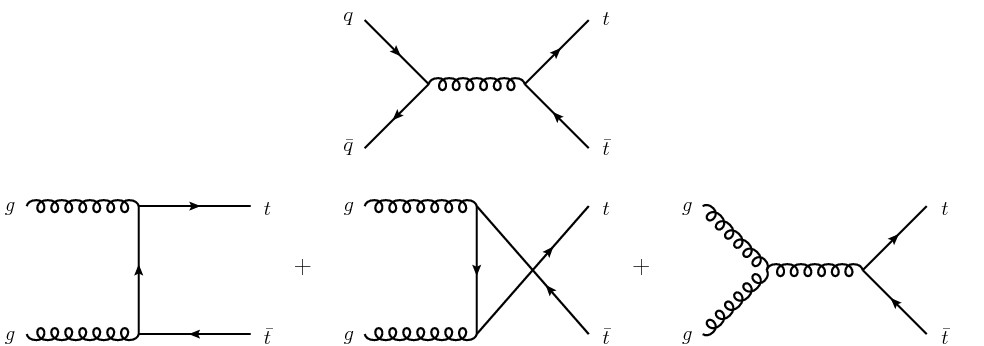
\includegraphics[width=0.97\textwidth]{figs/top-physics/ttbar_feyn.jpg}
\caption{The three Leading Order Feynman diagrams for top quark pair production at hadron colliders. Quark-anti quark annihilation is illustrated on the top row and gluon fusion on the bottom. Gluon fusion is the main production mode at the LHC and pair production at the Tevatron.}
\label{fig:feyn_ttbar}
\end{center}
\end{figure}

At the LHC the dominant mode of production is through gluon fusion, with quark-anti quark annihilation and the decay of the neutral photon and $Z^{0}$ bosons having smaller cross-sections~\cite{Shibata:2008sy}.

\subsection{Single top quark production}\label{subsec:singleTopTheory}


%%% QCD 2017
Single top quark production is a powerful probe between the top quark and electroweak sector, allowing for precision measurements of SM parameters whilst being sensitive to new physics, such as anomalous couplings.
Measuring single top quark processes is also important as such processes are backgrounds for Higgs and BSM physics searches and can be used to constrain Parton Distribution Functions (PDFs).	
%%%

The main SM single top production processes are categorised by the virtuality of the W boson involved in the interaction (see Fig.~\ref{fig:singleTopDiagrams}).

\begin{figure}[!h]
\centering
%%\includegraphics[width=0.47\textwidth]{figs/singleTopDiagrams.jpg}

\includegraphics[width=0.47\textwidth]{CMS-bw-logo.pdf}
\caption{Leading order diagrams for single top quark production channels via weak processes: (a) s-channel, (b) t-channel and (c) tW.}
\label{fig:singleTopDiagrams}
\end{figure}

Singly produced top quarks are produced through weak interactions by three differing channels, as shown in Fig.~\ref{fig:feyn_singletop}).
Such processes are an excellent probe of the SM as they allow the direct measurement of the $\abs{V_{tb}}$ element of the Cabibbo-Kobayashi-Maskawa (CKM) matrix as the top quark predominately decays to a bottom quark and thus test whether the CKM matrix is indeed unitary as presumed, or otherwise~\cite{Shibata:2008sy}.

\begin{figure}[htbp]
\begin{center}
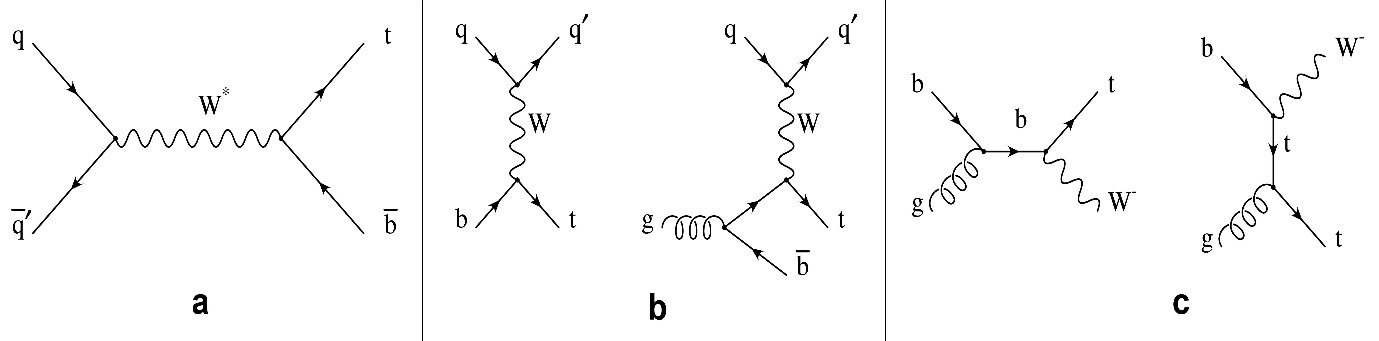
\includegraphics[width=1.00\textwidth]{figs/top-physics/singletop_feyn.jpg}
\caption{Feynman diagrams of single top production channels: a) s-channel; b) t-channel; c) tW-channel.}
\label{fig:feyn_singletop}
\end{center}
\end{figure}




Top quark pair production in association with a $\gamma$, $Z^{0}$, and $W^{\pm}$ vector bosons, are all expected to have a similar cross section and can be used to test the consistency of the SM and search for Beyond the SM (BSM) physics.
These channels, despite their small cross-sections, are important backgrounds which need to be understood in order to be able to probe for new physics with similar or smaller cross sections, such as $\ttbar$H\~cite{Khachatryan:2014ewa}.

\subsection{Single top production in association with a Z boson}\label{subsec:tZqTheory}

The production of a single top quark in association with a $Z^{0}$ boson with an additional jet (tZq), is a single top channel of interest.
This is a rare SM process that is based on single top production in the t-channel. The $Z^{0}$ boson is radiated off one of the quark legs, or from an exchanged W boson (Figure~\ref{fig:feyn_tZq}).
A greater understanding of the behaviour of this background is paramount to searches for BSM physics as this process is an irreducible background for many such searches of new physics (such as for Flavour Changing Neutral Current processes)~\cite{Quadt}. 

\begin{figure}[p]
\centering
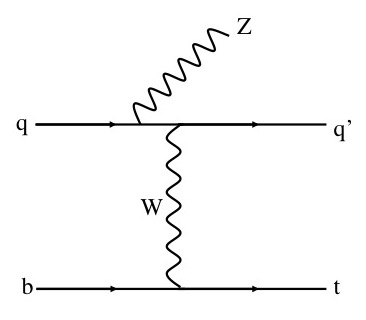
\includegraphics[width=0.47\textwidth]{figs/top-physics/tZq_feyn1.jpg}
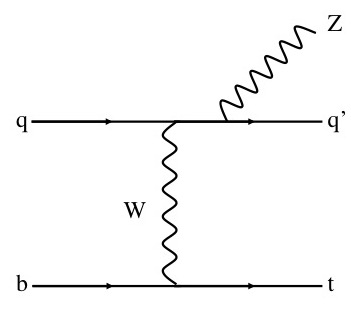
\includegraphics[width=0.47\textwidth]{figs/top-physics/tZq_feyn2.jpg}
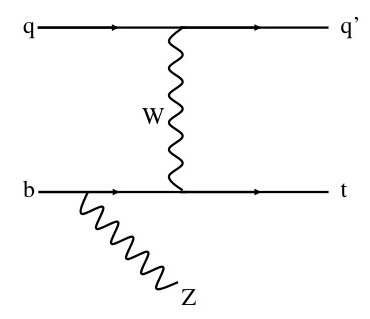
\includegraphics[width=0.47\textwidth]{figs/top-physics/tZq_feyn3.jpg}
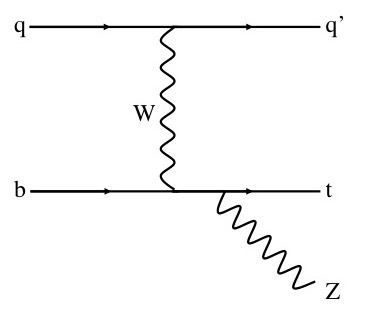
\includegraphics[width=0.47\textwidth]{figs/top-physics/tZq_feyn4.jpg}
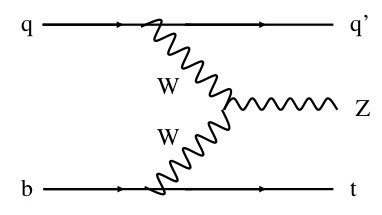
\includegraphics[width=0.47\textwidth]{figs/top-physics/tZq_feyn5.jpg}
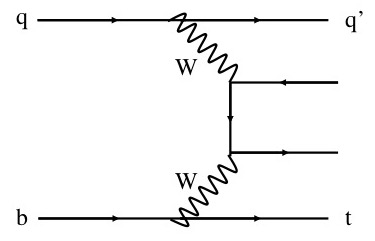
\includegraphics[width=0.47\textwidth]{figs/top-physics/tZq_feyn6.jpg}
\caption{Leading order tZq production diagrams. Diagram (f) represents the non-resonant contribution to the tqZ process.}
\label{fig:feyn_tZq}
\end{figure}

Prior to the first run of the LHC, proton-antiproton data for the top quark was collected at the Tevatron during both Run-I (at a centre-of-mass energy of 1.8 TeV) and Run-II (at a centre-of-mass energy of 1.96 TeV), corresponding to an integrated luminosity of 8.7 \fbinv.
The \ttbar production (di-lepton, lepton+jets and all-jets) cross section was within 9\% of the expected SM result~\cite{Lister:2008it} and the measurement of the top quark’s mass had a relative precision of 0.75\%~\cite{Group:2009ad}.
The Tevatron also found both the first evidence for the production of single top quarks~\cite{Abazov:2006gd} as well as discovering the production channel and from the measured cross-section, both collaborations were able to directly determine the CKM matrix element which describes the Wtb coupling and determine that it had a 95\% confidence level of being consistent with the SM~\cite{Aaltonen:2009jj}.

During 2012, $19.7\pm0.5 \fbinv$ at a centre-of-mass energy of 8 TeV (roughly four times larger than the 7 TeV data) was collected by the CMS Collaboration at the LHC. 
Analysis of the top quark pair production cross-section is generally in good agreement with the SM predictions at next-to-next-to-leading order (NNLO). 
The pT spectrum for data for leptons, jets and top quarks however, is softer than the predictions and similarly to CMS measurements at 7\TeV, the NLO+NNLO calculations fails to describe the data for all $\pT^{\ttbar}$ values~\cite{Khachatryan:2015oqa}. 
Measurements of the W boson helicity fractions from the decay of a single top quark, at centre-of-mass energies of 8 TeV, are in agreement with the SM predictions at NNL0  and have a similar precision to the W boson helicity fractions measurements from top quark pair production at 7 TeV at the LHC~\cite{Khachatryan:2014vma}.

At the LHC, for proton-proton collisions at 8 TeV the predicted cross-section at next-to-leading order (NLO) for SM tZ production is~\cite{Campbell:2013yla}:

\begin{equation}
\sigma(tZ)= 160_{-2}^{+7} (scale)_{-11}^{+11} (PDF) fb \;.
\sigma(\bar{t}Z)= 76_{-1}^{+4} (scale)_{-5}^{+5} (PDF) fb \;.
\end{equation}

This leads to an overall cross-section of $236_{-16}^{+19}$ fb. 
These cross-sections were determined using the CTEQ6M set of Parton Distribution Functions (PDF)~\cite{Pumplin:2002vw}. 
The $\bar{t}$Z cross-section is roughly half that of the tZ cross-section due to the ratio of the up quark PDF to the down quark PDF is circa 0.5 in the x range typical for these processes\cite{Campbell:2013yla}. 
The CMS collaboration have measured the $\ttbar$Z cross-section to be\cite{Khachatryan:2014ewa}

\begin{equation}
\sigma (\ttbar Z)= 200_{-70}^{+80} (statistics)_{-30}^{+40} (systematics) fb \;.
\end{equation}

The cross-section between $\ttbar$Z and the sum of the tZ and $\bar{t}$Z cross-sections is comparable as whilst single top + Z processes are electroweak interactions (in contrast to the QCD-induced top quark pair production) they have fewer daughters in the final state and the Z boson condition for $\ttbar$Z considerably reduces the rate\cite{Campbell:2013yla}.
As such, a search for tZ processes should be achievable during CMS Run-1 data. This is supported by CMS’ Run-I results for $\ttbar$Z~\cite{Khachatryan:2014ewa}. 
A CMS Analysis Note and a journal paper supporting a three sigma probability of evidence of single top production in association with a Z boson and a jet are currently being produced by the HEP Group at Brunel University London~\cite{Sirunyan:2017kkr}.

Until now, the 2012 data taken at 8 TeV, has been used by the research group to analyse these processes.
Following the restart of the LHC after the phase-0 upgrades, new data are anticipated to be available with the increase to a higher centre-of-mass energy and with anticipated luminosities of up to 3000~\fbinv\cite{ECFA}. 
Such statistics will be used to gain more precise measurements of top quark pair production and the production of single top quarks and as a result, a better understanding of the underlying processes involved.

\section{Beyond The Standard Model}\label{sec:bsm}
The SM has been an incredibly successful theory
Despite the incredible successes of the SM however, there  

 in terms of both its predictive powers and ability to accurately describe the majority of the properties of the known fundamental particles up to the electroweak scale, it is clear that the SM is far from being a complete theory. 

As 

One of the most apparent shortcomings of the SM is the lack of an explanation for why we observe an asymmetry in the quantities of matter and anti-matter in the observable universe.

Andrei Sakharov 

Aside from electroweak symmetry breaking, there are a number of other fundamental phenomena that the SM does not account for. 

The most ...  

These include, but are not limited to, the lack of explanation for gravity, the lack of candidates for dark matter, and observed matter/antimatter asymmetry in the universe. 
Gravity is left unexplained as the SM, a quantum mechanical theory, is incompatible with General Relativity, a classical theory~\cite{Khalil:2003vd}. 



There are many 
Supersymmetry (SUSY), a popular extension of the SM, makes progress with these questions by proposing that every fundamental fermion has a massive boson ``superpartner'' (and vice versa for the gauge bosons). 
The superpartners generalise space-time symmetries, allowing for bosons and fermions to be related, a straightforward unification of the strengths of the weak, electromagnetic and strong interactions at high energies and a more ``natural'' emergence of the Higgs potential~\cite{Khalil:2003vd}. 
These supersymmetric particles' (sparticles) spin differs from their SM counterparts by 1/2 (\ie bosons' supersymmetric partners are fermions, and vice versa). 
As supersymmetry is ``broken'', the expected sparticle masses are considerably greater than their equivalent partner masses. 

Additionally, some SUSY models also include candidates for a dark matter particle which is consistent with observations. 
However, while superpartners should be observed at the LHC if SUSY exists at the electroweak scale, no superpartner has been observed so far, with results being used to constrain the range of the possible superpartner masses. 
If SUSY, in any of its forms, exists, then higher energy runs of the LHC will be required to illuminate it.

%% INTRO BIT
%The SM has been one of the greatest and most powerful scientific theories, making remarkably accurate predictions which have withstood incredible experimental scrutiny.
%Despite the completion of the SM with the discovery of the Higgs Boson in 2012~\cite{HiggsCMS,HiggsATLAS} at the Large Hadron Collider (LHC), it is clear that the Standard Model cannot be a complete description of reality:
%\begin{itemize}
%\item Gravity is not accounted for by the quantum field theory of the SM and at high energy densities it is fundamentally irreconcilable with the classical theory of General Relativity~\cite{}.
%\item There is strong experimental evidence that the observed galaxy rotation curves and gravitational lensing cannot be accounted for by SM particles and that there must be a large weakly interacting \emph{Dark Matter} component of the Universe~\cite{Bertone:2004pz}.
%\item The presence of a \emph{Dark Energy} energy has also been inferred from astronomical and cosmological observations to account for the observed rate of expansion of the Universe~\cite{Peebles:2002gy}.
%\item Neutrinos have been observed to oscillate between different flavours, implying that they have non-zero masses in contrast to the SM~\cite{Fukuda:1998mi,Ahmad:2001an}.
%\item There is currently no explanation that accounts for the clear abundance of matter over anti-matter in the observable universe.
%\item On top of the abovce inconsistencies, many scientists are uncomfortable with the fact that the SM contains a large number of finely tuned experimentally derived parameters and hope that these values would emerge naturally from a more ``complete'' description of reality~\cite{}.
%\end{itemize}
